\documentclass[10pt, conference, compsocconf]{IEEEtran}

\usepackage{tikz}
\usetikzlibrary{shapes.geometric, arrows}
\usepackage{multirow}
\usepackage{graphicx}
\graphicspath{../results/roc-nn-keras}

\hyphenation{}

\begin{document}
\title{Software Fault Prediction using Artificial Neural Networks}

\author{
  \IEEEauthorblockN{Prajwal D Prakash}
  \IEEEauthorblockA{Dept. of CS\&E\\
    BMSIT\&M\\
    Bangalore\\
    Email: prajwalpy6@gmail.com}
  \and
  \IEEEauthorblockN{Gaurav Vattikuti}
  \IEEEauthorblockA{Dept. of CS\&E\\
    BMSIT\&M\\
    Bangalore\\
    Email: vattikutigaurav@gmail.com}
  \and
  \IEEEauthorblockN{Yeresime Suresh}
  \IEEEauthorblockA{Dept. of CS\&E\\
    BMSIT\&M\\
    Bangalore\\
    Email: ysuresh@bmsit.in}
}
\maketitle

\begin{abstract}
  Software faults are dangerous. Software systems are often essential to a business operation or organization and failures in such systems cause disruption of some goal directed activity (mission critical). Malfunctions in other safety-critical systems may result in death, loss of property or environmental harm. Most damaging software malfunctions are run-time malfunctions that are not always caught during the testing process. In such cases, predicting software faults before they occur, gives designers an insight to the possible malfunctions and the relative probability of their occurrence. This helps in focused testing and saves time during the software development life cycle. The artificial neural network is a powerful tool for the detection of faults due to its ability to differentiate between various patterns. This paper presents the design and development of artificial neural network based model for software fault detection in context of fault-prone modules.
\end{abstract}

\begin{IEEEkeywords}
  software fault detection; artificial neural networks;
\end{IEEEkeywords}

\IEEEpeerreviewmaketitle

\section{Introduction}
There has been a tremendous growth in the demand for software quality during recent years. As a consequence, issues related to testing are becoming increasingly crucial. The ability to measure software fault-proneness can be extremely important for minimizing cost and improving the overall effectiveness of the testing process. The majority of faults in a software system are found in a few of its com- ponents (Boehm and Papaccio, 1988; Porter and Selby, 1990). The ``80:20'' rule states that approximately 20\% of a software system is responsible for 80\% of its errors, costs, and rework (Boehm, 1987). Boehm and Papaccio (1988) conclude:
\begin{quote}
  ``The major implication of this distribution is that software verification and validation activities should focus on identifying and eliminating the specific high-risk problems to be encountered by a software project, rather than spreading their available early-problem-elimination effort uniformly across trivial and severe problems.''
\end{quote}
Therefore, the possibility of estimating the potential faultiness of software components at an early stage can be of great help for planning testing activities. For example, testing effort can be focused on a subset of software components (e.g., the potentially ``most troublesome'' 20\%). Unfortunately, software fault-proneness cannot be directly measured. However, it can be estimated based on software metrics, which provide quantitative descriptions of program attributes.

\section{Literature Survey}

Table \ref{tab:literature-survey} shows the relevant literature survey.

\begin{table*}[t]
  \centering
  \caption{Literature Survey}
  \label{tab:literature-survey}
  \begin{tabular}{|p{5cm}|p{3cm}|p{1cm}|p{3cm}|p{2cm}|p{2cm}|}
    \hline
    \textbf{Paper Title} & \textbf{Authors} & \textbf{Year of Publication} & \textbf{Method Proposed} & \textbf{Data-set Used} & \textbf{Results Obtained} \\ \hline
    \multirow{2}{5cm}{Comparative analysis of neural network and genetic programming for number of software faults prediction \cite{paper1}} &
    \multirow{2}{3cm}{Santosh Singh Rathore, Sandeep Kuamr} &
    \multirow{2}{1cm}{2015} &
    \multirow{2}{3cm}{Generic method better than neural networks.} &
    Camel 1.4 & 143.47\% completeness \\ \cline{5-6}
    & & & & Camel 1.2 & 69.10\% completeness \\ \hline

    \multirow{5}{5cm}{Applying swarm ensemble clustering technique for fault prediction using software metrics \cite{paper2}} &
    \multirow{5}{3cm}{Rodrigo A. Coelho, Fabrício dos R. N. Guimarães, Ahmed A. A. Esmin} &
    \multirow{5}{1cm}{2014}
    & K-means with the Euclidean similarity function (KM-E)  & CM1 (KM-E) & 83.94\% accuracy \\ \cline{4-6}
    & & & K-means with the Manhattan similarity function (KM-M) & CM1 (EM)  & 81.33\% accuracy \\ \cline{4-6}
    & & & PSO clustering with the Euclidean similarity function (PSO-E) & CM1 (EM) & 70.29\% accuracy \\ \cline{4-6}
    & & & PSO clustering with Manhattan similarity function (PSO-M) & CM1 (PSO-E) & 89.96\% accuracy \\ \cline{4-6}
    & & & Expectation–maximization clustering algorithm (EM) & CM1 (PSO-M) & 71.29\% accuracy \\ \hline
    \multirow{3}{5cm}{Supplementing Object-Oriented software change impact analysis with fault-proneness prediction \cite{paper3}} &
    \multirow{3}{3cm}{Bassey Isong, Ohaeri Ifeoma, Munienge Mbodila} &
    \multirow{3}{1cm}{2016} &
    \multirow{3}{3cm}{NASA KC1, 3 sets of predictors {[}m1,m2,m3{]}}
    & M1 & 97\% training accuracy\\ \cline{5-6}
    & & & & M2 & 90\% training accuracy \\ \cline{5-6}
    & & & & M3 & 99\%,training accuracy \\ \hline
    \multirow{1}{5cm}{A model for early prediction of faults in software systems \cite{paper4}} &
    \multirow{1}{3cm}{Parvinder S. Sandhu, Amanpreet S. Brar, Raman Goel, Jagdeep Kaur, Sanyam Anand} &
    \multirow{1}{1cm}{2010} &
    Decision tree based Model in combination of K-means clustering as pre-processing technique & CM1 & 100\% on 10-fold cross validation \\ \hline
    \multirow{4}{5cm}{Artificial neural network-based metric selection for software fault-prone prediction model \cite{paper5}} &
    \multirow{4}{3cm}{C. Jin, S.-W. Jin, J.-M. Ye} &
    \multirow{4}{1cm}{2012}
    & DT & PC1 & 94.14\% accuracy \\ \cline{4-6}
    & & & SFPM & CM1 & 91.17\% accuracy \\ \cline{4-6}
    & & & SFPM & KC1 & 87.74\% accuracy \\ \cline{4-6}
    & & & LR & KC3 & 93.42\% accuracy \\ \hline
  \end{tabular}
\end{table*}

\section{Methodology}
The field of machine learning focuses on the study of algorithms that improve their performance at some task automatically through experience (Mitchell, 1997). An artificial neural network (ANN) is an efficient information processing system which resembles in characteristics with a biological neural network. ANN’s possess large number of highly interconnected processing elements called neurons. Each neuron is connected with the other by a connection link. Each connection link is associated with weights which contain information about the input signal. This information is used by the neuron net to solve a particular problem. Each neuron has an internal state of its own. This internal state is called the activation level of neuron, which is the function of the inputs the neuron receives. There are a number of activation functions that can be applied over net input such as Gaussian, Linear, Sigmoid and Tanh. It is the Sigmoid function that is the most frequently used in neural nets. Thus, the models of ANN are specified by the three basic entities namely:

\begin{enumerate}

\item The model’s synaptic interconnections;
\item The training or learning rules adopted for updating and adjusting the connection weights;
\item Their activation functions.

\end{enumerate}

The neural network process starts by developing the structure of the network and establishing the technique used to train the network using an existing data set. Neural network architectures are divided into two groups:

\begin{enumerate}
\item Feed forward networks where no loops in the network path occur.
\item Feedback networks that have recursive loops.

\end{enumerate}

The most common architecture of neural networks which is used in software cost estimation is the Back-Propagation trained Feed Forward networks. The training algorithm of back propagation involves four stages:

\begin{enumerate}
\item Initialization of weights
\item Feed forward
\item Back Propagation of errors
\item Updating of the weights and biases
\end{enumerate}

\section{Data-set and Metrics}
In this section, we present a brief description of the software fault dataset, software metrics and evaluation metrics used for analysis.

\subsection{Data-set}
The camel-1.6 data-set is used for the experimental evaluation of our model, which has been collected from the PROMISE data repository\cite{promisedataset}. The data-set is an analysis of 92 versions of 38 proprietary, open-source and academic projects. The data-set contains a record of twenty object-oriented metrics and the number of faults found in the software system during testing and after the release.

The camel-1.6 data-set has 965 total number of modules, with 188 faulty modules, each with a given number of faults. In our setup, we only classify whether a module is faulty. Therefore, the number of faults in the module is not taken into account.

\subsection{Used Metrics}
The camel-1.6 data-set uses the Chidamber \& Kemerer object-oriented metrics. These Metrics were designed to measure the complexity of an object-oriented modelled design. Though the data-set uses twenty metrics, we use only the metrics the suite originally consisted of. These 6 metrics are calculated for each class: WMC (Weighted Methods Per Class), DIT (maximum inheritance path from the class to the root class), NOC (number of immediate sub-classes of a class), CBO (number of classes to which a class is coupled), RFC (Response for a Class) and LCOM1 (Lack of Cohesion of Methods).

\subsection{Metrics for evaluation of classifiers}
The experimental evaluation of such a model is performed according to several performance metrics, such as probability of detection (PD), probability of false alarm (PF), balance, or area under the ROC (Receiver Operating Characteristics) curve.

The following set of evaluation measures are being used to find the results:

\begin{enumerate}
\item

  Probability of Detection (PD), also called recall or specificity, is the probability of correct classification of a module that contains a fault.

  \begin{equation}
    PD = recall = \frac{TP}{TP + FN}
  \end{equation}

\item

  Probability of False Alarms (PF) is the ratio of false positives to all non defect modules.

  \begin{equation}
    PF = \frac{FP}{FP + TN}
  \end{equation}

\item

  The accuracy of the model is the probablity of the correct classification of a module.

  \begin{equation}
    Accuracy = \frac{TN + TP}{TN + FP + FN + TP}
  \end{equation}

\item

  The precision is the ability of the classifier not to label as positive a sample that is negative.

  \begin{equation}
    Precision = \frac{TP}{TP + FP}
  \end{equation}

\item

  The F-measure can be interpreted as a weighted harmonic mean of the precision and recall.

  \begin{equation}
    F-measure = \frac{2 * precision * recall}{precision + recall}
  \end{equation}

\item

  ROC(Receiver Operator Characteristic) is a plot of PD versus PF across all possible experimental combinations.

\end{enumerate}

In Table \ref{tab:confusion-table}, a confusion matrix is calculated after N*M cross-validation.

\begin{table}[]
  \centering
  \begin{tabular}{l|l|l|}
    \cline{2-3}
    & NO (Prediction)     & YES (Prediction) \\ \hline
    \multicolumn{1}{|l|}{NO (Actual)}  & TN (True Negative)  & FP (False Positive)  \\ \hline
    \multicolumn{1}{|l|}{YES (Actual)} & FN (False Negative) & TP (True Positive)  \\ \hline
  \end{tabular}
  \caption{Confusion Table}
  \label{tab:confusion-table}
\end{table}

\section{Implementation and Results}
The neural network is implemented using Keras\cite{keras} running on top of Theano. The Keras Sequential model is set up as shown in figure \ref{fig:nn-architecture}.

\tikzstyle{block} = [rectangle, draw, text width=20em, text centered, minimum height=1.5em]
\tikzstyle{line} = [draw, -latex']

\begin{figure}
  \centering
  \begin{tikzpicture}[node distance = 1cm, auto]

    \node [block] (1) {dense 0 - input layer (6 nodes)};
    \node [block, below of=1] (2) {dense 1 - hidden layer 1 (50 nodes)};
    \node [block, below of=2, text width=10em] (3) {activation 1 - $relu$};
    \node [block, below of=3] (4) {dense 2 - hidden layer 2 (70 nodes)};
    \node [block, below of=4, text width=10em] (5) {activation 2 - $relu$};
    \node [block, below of=5] (6) {dense 3 - hidden layer 2 (90 nodes)};
    \node [block, below of=6, text width=10em] (7) {activation 3 - $relu$};
    \node [block, below of=7] (8) {dense 4 - output layer (1 node)};
    \node [block, below of=8, text width=10em] (9) {activation 3 - $sigmoid$};

    \path [line] (1) -- (2);
    \path [line] (2) -- (3);
    \path [line] (3) -- (4);
    \path [line] (4) -- (5);
    \path [line] (5) -- (6);
    \path [line] (6) -- (7);
    \path [line] (7) -- (8);
    \path [line] (8) -- (9);
  \end{tikzpicture}

  \caption{The architecture of the ANN}
  \label{fig:nn-architecture}
\end{figure}

It was concluded that the architecture (in figure \ref{fig:nn-architecture}) performed the best for the camel-1.6 dataset. The neural network has three hidden layers. The input layer has 6 nodes, one for each CK Metric class. The first hidden layer has 50 nodes, the second hidden layer has 70 nodes and the third hidden layer has 90 nodes. The implementation is a binary classification. The activation function used is $ReLU$, i.e. rectified linear unit function for both the hidden layers and $sigmoid$, i.e the exponential function for the output layer. The $ReLU$ activation function's output ranges from -1 to 1 and is better suited for the normalized input from the normalization layer that has a mean close to 0, and a standard deviation close to 1. The $ReLU$ function is also known to be faster than $tanh$, i.e. the hyperbolic tangent function \cite{relufaster}. The $sigmoid$ function is suited for a binary classification like the one in our setup, because it produces output probabilities in the range [0, 1]. The optimizer used was $Adagrad$ and the loss considered was $binary crossentropy$.

\subsection{Results}
The result obtained on 10-fold cross validation is shown in \ref{tab:results}.

\begin{table}[]
  \centering
  \begin{tabular}{l|l|l|}
    \cline{2-3}
    & NO (Prediction)     & YES (Prediction) \\ \hline
    \multicolumn{1}{|l|}{NO (Actual)}  & 77 (True Negative)  & 3 (False Positive)  \\ \hline
    \multicolumn{1}{|l|}{YES (Actual)} & 12 (False Negative) & 4 (True Positive)  \\ \hline
  \end{tabular}
  \caption{Results}
  \label{tab:results}
\end{table}

The accuracy obtained on the above fold was 84.36\% with a good AUC of 0.8. The ROC Curve is shown in figure \ref{fig:roc}.

\begin{figure}[h]
\centering
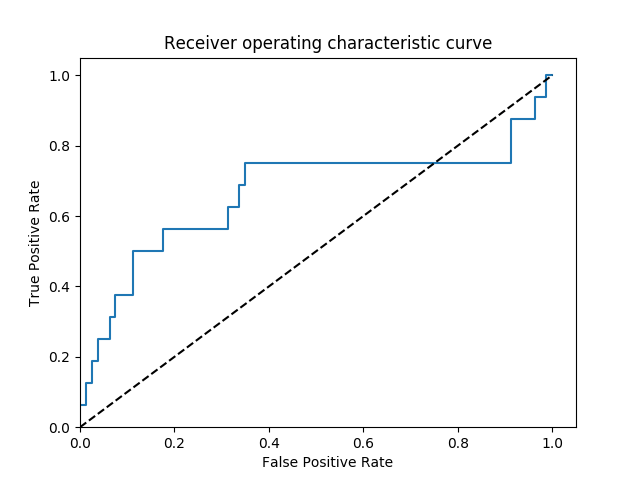
\includegraphics[width=8cm]{fold_09.png}
\caption{Receiver Operator Characteristic Curve}
\label{fig:roc}
\end{figure}

\section{Conclusion}
The conclusion goes here. this is more of the conclusion

\section*{Acknowledgment}

\begin{thebibliography}{1}
\bibitem{promisedataset} Menzies, T., Krishna, R., Pryor, D. (2016). The Promise Repository of Empirical Software Engineering Data; { \em http://openscience.us/repo }. North Carolina State University, Department of Computer Science
\bibitem{keras} Keras, a high-level neural networks library, written in Python; { \em https://keras.io/ }
\bibitem{paper1} Rathore, Santosh Singh, and Sandeep Kuamr. "Comparative analysis of neural network and genetic programming for number of software faults prediction." Recent Advances in Electronics \& Computer Engineering (RAECE), 2015 National Conference on. IEEE, 2015.
\bibitem{paper2} Coelho, Rodrigo A., Fabrício dos RN Guimarães, and Ahmed AA Esmin. "Applying swarm ensemble clustering technique for fault prediction using software metrics." Machine Learning and Applications (ICMLA), 2014 13th International Conference on. IEEE, 2014.
\bibitem{paper3} Isong, Bassey, Ohaeri Ifeoma, and Munienge Mbodila. "Supplementing Object-Oriented software change impact analysis with fault-proneness prediction." Computer and Information Science (ICIS), 2016 IEEE/ACIS 15th International Conference on. IEEE, 2016.
\bibitem{paper4} Sandhu, Parvinder S., et al. "A model for early prediction of faults in software systems." Computer and Automation Engineering (ICCAE), 2010 The 2nd International Conference on. Vol. 4. IEEE, 2010.
\bibitem{paper5} Jin, Cong, S-W. Jin, and J-M. Ye. "Artificial neural network-based metric selection for software fault-prone prediction model." IET software 6.6 (2012): 479-487.
\bibitem{relufaster} Alex Krizhevsky, Ilya Sutskever, Geoffrey E. Hinton, “ImageNet Classification with Deep Convolutional Neural Networks” http://www.cs.toronto.edu/ fritz/absps/imagenet.pdf
\end{thebibliography}

\end{document}
